
% asset_id: FAS1VectorsTikZ-004
% asset_type: tikz
% topic_id: FAS1Vectors
% unit_code: FAS1
% topic_code: FAS1-VEC
% related_lesson_file: FAS1_vectors_lesson.md
% related_lesson_section: # 9. Visual Asset Integration
% source: FP1-Chp1-Vectors.pdf + transcripts.md where relevant
\documentclass[tikz,border=8pt]{standalone}
\usepackage{amsmath}
\usepackage{xcolor}
\usetikzlibrary{arrows.meta,calc,positioning}
\definecolor{Canvas}{HTML}{FAF9F6}
\definecolor{Ivory}{HTML}{FFFFF0}
\definecolor{LineGrey}{HTML}{E5E5EA}
\definecolor{Gold}{HTML}{C5A059}
\definecolor{TextInk}{HTML}{2C2C2E}
\definecolor{SoftPink}{HTML}{FBEFEF}
\begin{document}
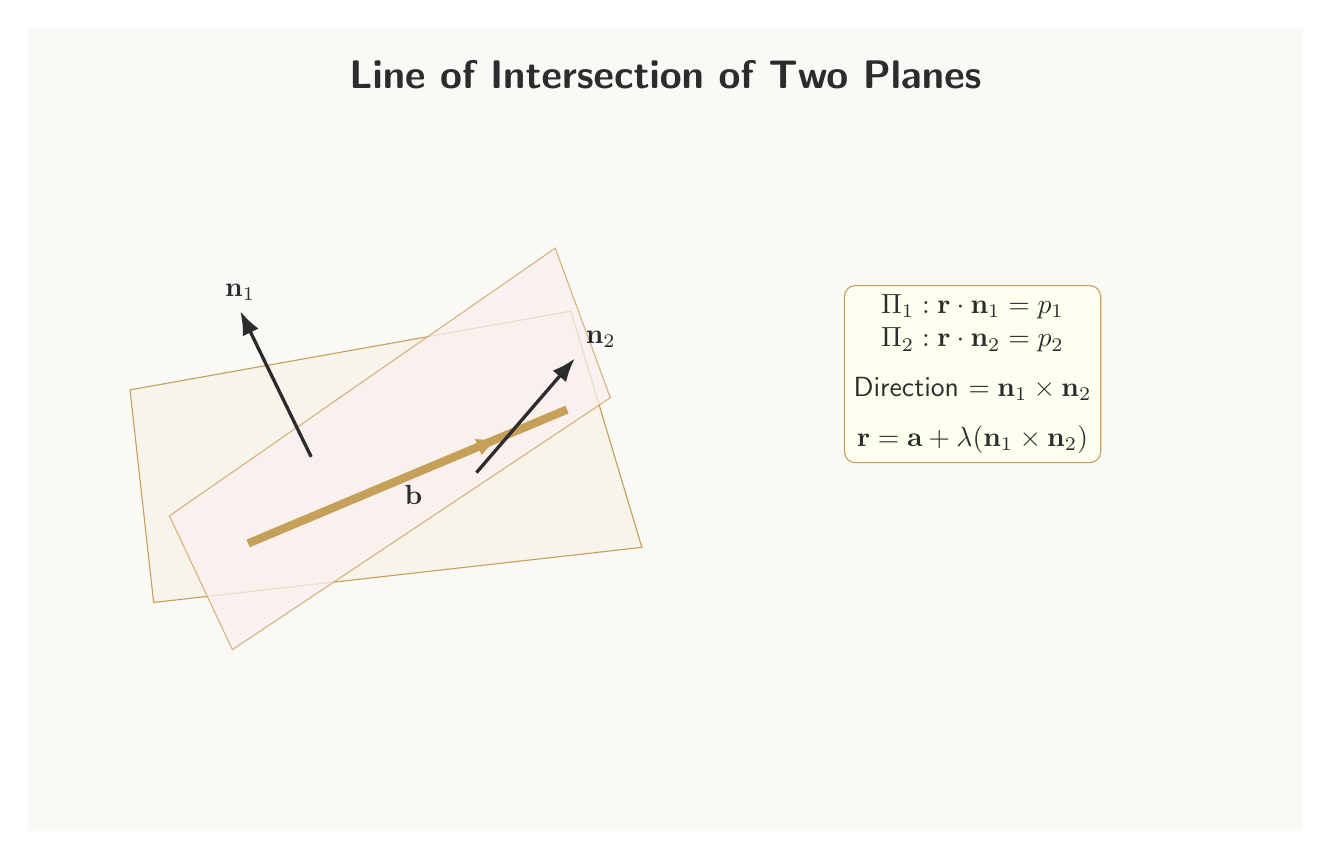
\begin{tikzpicture}[every node/.style={font=\sffamily,text=TextInk},arrow/.style={-{Latex[length=3mm]},line width=1.2pt,draw=TextInk},goldarrow/.style={-{Latex[length=3mm]},line width=1.5pt,draw=Gold}]
\fill[Canvas] (-0.6,-0.6) rectangle (15.6,9.6);

\node[font=\sffamily\bfseries\Large] at (7.5,9) {Line of Intersection of Two Planes};
\filldraw[fill=Gold!12,draw=Gold] (1,2.3)--(7.2,3)--(6.3,6)--(0.7,5)--cycle; \filldraw[fill=SoftPink,draw=Gold,opacity=.75] (2,1.7)--(6.8,4.9)--(6.1,6.8)--(1.2,3.4)--cycle;
\draw[Gold,line width=3pt] (2.2,3.05)--(6.25,4.75); \draw[goldarrow] (3.2,3.47)--(5.4,4.39) node[midway,below] {$\mathbf b$};
\draw[arrow] (3.0,4.15)--++(-0.9,1.85) node[above] {$\mathbf n_1$}; \draw[arrow] (5.1,3.95)--++(1.25,1.45) node[above right] {$\mathbf n_2$};
\node[draw=Gold,fill=Ivory,rounded corners,align=center] at (11.4,5.2) {$\Pi_1:\mathbf r\cdot\mathbf n_1=p_1$\\$\Pi_2:\mathbf r\cdot\mathbf n_2=p_2$\\[6pt]Direction $=\mathbf n_1\times\mathbf n_2$\\[6pt]$\mathbf r=\mathbf a+\lambda(\mathbf n_1\times\mathbf n_2)$};

\end{tikzpicture}
\end{document}
